\documentclass[]{book}

\usepackage{array,epsfig}
\usepackage{amsmath}
\usepackage{amsfonts}
\usepackage{amssymb}
\usepackage{amsxtra}
\usepackage{amsthm}
\usepackage{mathrsfs}
\usepackage{color}

\usepackage{hyperref}
\hypersetup{colorlinks=false}

\theoremstyle{definition}
\newtheorem{defn}{Definition}
\newtheorem{thm}{Theorem}
\newtheorem{cor}{Corollary}
\newtheorem*{rmk}{Remark}
\newtheorem*{lem*}{Lemma}
\newtheorem{lem}{Lemma}
\newtheorem*{joke}{Joke}
\newtheorem{ex}{Example}
\newtheorem*{soln}{Solution}
\newtheorem{prop}{Proposition}

\setlength{\topmargin}{-.3 in}
\setlength{\oddsidemargin}{0in}
\setlength{\evensidemargin}{0in}
\setlength{\textheight}{9.in}
\setlength{\textwidth}{6.5in}
\pagestyle{empty}

\newcommand{\x}{\mathbf{x}}
\newcommand{\y}{\mathbf{y}}
\newcommand{\z}{\mathbf{z}}
\newcommand{\0}{\mathbf{0}}



\begin{document}

\begin{center}
{\Large\textbf Math 20250 \hspace{0.5cm} Midterm 1}\\
\large{Alex Sheng}\\
\normalsize{Due: Friday Oct 23, 11:59 PM}
\end{center}

\vspace{0.2 cm}

\noindent First I shall prove a lemma that later I will invoke later:

\begin{lem*}\label{lemma}
Let $A:V\to W$ be a linear transformation and $v_1,v_2,...,v_n$ a set of basis in $V$, then $f$ is an isomorphism iff $A(v_1),A(v_2),...,A(v_n)$ forms a basis in $W$.
\end{lem*}
\begin{proof}
The direction ``isomorphism $\Rightarrow$ basis" I proved correctly in Homework 2:\newline
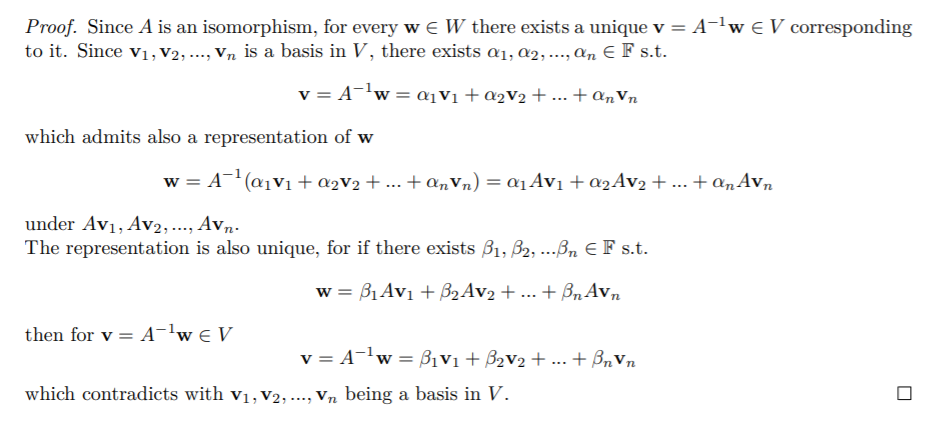
\includegraphics[scale=1]{images/mid.jpg}\smallbreak
\noindent For the other direction, construct $g:W\to V$ s.t. $g:A(v_i)\mapsto v_i$. It's easy to see that $g$ is an invertible linear transformation. Indeed, $\forall v\in V$
\[g\circ A(v)=g\circ A(\sum_{i=1}^n\alpha_iv_i)=g(\sum_{i=1}^n\alpha_iw_i)=v=\textrm{Id}_V\]
and same goes for $A\circ g=\textrm{Id}_W$.
\end{proof}

\bigbreak

\begin{enumerate}
\item Problem 1. (20 points)
\begin{soln} with 2 pivots:$
\begin{pmatrix}
1 & 0\\
0 & 1
\end{pmatrix}$\newline
with 1 pivot: $\begin{pmatrix}
1 & a\\
0 & 0
\end{pmatrix}, \begin{pmatrix}
0 & 1\\
0 & 0
\end{pmatrix}$\newline
with 0 pivot (vacuously true): $\begin{pmatrix}
0 & 0\\
0 & 0
\end{pmatrix}$
\end{soln}

\item Problem 2. (20 points)
\begin{soln}
Let $v_1=\begin{pmatrix}
1 & 0\\
0 & 0
\end{pmatrix},v_2=\begin{pmatrix}
1 & 1\\
0 & 0
\end{pmatrix},v_3=\begin{pmatrix}
0 & 0\\
1 & 1
\end{pmatrix},v_4=\begin{pmatrix}
0 & 0\\
0 & 1
\end{pmatrix}$.\newline 
Note that $v_i^2=v_i$ for $i=1,2,3,4$\newline
They are linearly independent:
\[av_1+bv_2+cv_2+dv_4=\begin{pmatrix}
a+b & b \\
c & c+d
\end{pmatrix}=\begin{pmatrix}
0 & 0\\
0 & 0
\end{pmatrix}\Rightarrow a=b=c=d=0\]
The are also generating:
\[\forall \begin{pmatrix}
m & n\\
p & q
\end{pmatrix}\in V:\begin{pmatrix}
m & n\\
p & q
\end{pmatrix}=(m-n)v_1+nv_2+pv_3+(q-p)v_4\]
\end{soln}
Hence $v_1$, $v_2$, $v_3$, and $v_4$ form a basis in $V$.

\item Problem 3. (20 points)
\begin{enumerate}
    \item (15 points)
    \begin{proof}
    Let $v_1$, $v_2$, and $v_3$ be a basis in $\mathbb{R}^3$. We will show that $UT(v_1)$, $UT(v_2)$, $UT(v_3)$ do \emph{not} form a basis in $\mathbb{R}^3$, which by \hyperref[lemma]{lemma}, implies that $UT$ is not invertible.\smallbreak
    Since in $\mathbb{R}^2$ there can't be more than 2 linearly independent vectors, $\exists\alpha,\beta$ s.t. $T(v_3)=\alpha T(v_1)+\beta T(v_2)$, then
    \[U(T(v_3))=U(\alpha T(v_1))+U(\beta T(v_2))\Rightarrow UT(v_3)=\alpha UT(v_1)+\beta UT(v_2)\]
    which shows that $UT(v_1)$, $UT(v_2)$, $UT(v_3)$ are not linearly independent. Hence they do not form a basis in $\mathbb{R}^3$.
    \end{proof}
    \item (5 points)
    Let $A=\begin{pmatrix}
    \alpha_1 & \alpha_2\\
    \alpha_3 & \alpha_4
    \end{pmatrix}$ and $B=\begin{pmatrix}
    \beta_1 & \beta_2\\
    \beta_3 & \beta_4
    \end{pmatrix}$.\newline
    Equation $AB=O_2$ yields restrictions on the choice of $\alpha$s and $\beta$s, namely
    \begin{equation}\label{(1)}
    \frac{\alpha_1}{\alpha_2}=\frac{\alpha_3}{\alpha_4}=-\frac{\beta_3}{\beta_1}=-\frac{\beta_4}{\beta_2}
    \end{equation}
    Now for $BA\neq O_2$ choose $\alpha$s and $\beta$s satisfying \hyperref[(1)]{(1)} and $\alpha_1\beta_1+\alpha_3\beta_2\neq 0$. For instance:
    \[A=\begin{pmatrix}
    5 & -10\\
    2 & -4
    \end{pmatrix},B=\begin{pmatrix}
    1 & 0.5\\
    0.5 & 0.25
    \end{pmatrix}\]
\end{enumerate}

\item Problem 4. (20 points)
\begin{soln}
From the solution given we know that $x_1=1$ and $x_4=0$, which gives us
\begin{equation*}
\begin{cases}
x_1+0x_2+0x_3+0x_4=1\\
0x_1+0x_2+0x_3+x_4=0
\end{cases}
\end{equation*}
Since there are 2 free variables and 4 unknowns, by rank-nullity theorem the last two equations should be the trivial ones. Since the problem asks for 3 equations, the result is
\begin{equation*}
\begin{cases}
x_1+0x_2+0x_3+0x_4=1\\
0x_1+0x_2+0x_3+x_4=0\\
0x_1+0x_2+0x_3+0x_4=0
\end{cases}
\end{equation*}
\end{soln}

\item Problem 5. (20 points)
\begin{proof}
Recall that dimension is the number of vectos in a basis.\smallbreak
If $\dim V=\dim W$, let $v_1,v_2,...,v_n$ and $w_1,w_2,...,w_n$ be a set of basis in $V$ and $W$ respectively. Construct a linear map $f:V\to W$ by $f:v_i\mapsto w_i$ for $i=1,2,...,n$. By \hyperref[lemma]{lemma} $f$ is an isomorphism, hence $V\cong W$.\smallbreak
On the other hand, if $\exists f:V\to W$ an isomorphism, by \hyperref[lemma]{lemma} it maps a set of basis in $V$ bijectively to that in $W$. Hence $\dim V=\dim W$.
\end{proof}


\end{enumerate}

\end{document}